\documentclass[final]{ltugboat}

% typeset with pdflatex (not latex & dvi) since figure is .pdf (so, in TeXShop, for instance, set Typeset > Pdftex )

\usepackage{url}

% original compilation yielded "\pdfendlink ended up in different nesting level than \pdfstartlink." error message,
% but fix on http://www.tug.org/errors.html recommended using draft option to hyperref:
%"This happens when hyperref is used under pdftex and a citation splits across a page boundary. To fix it, note the page number of the error and specify the draft option to hyperref so you get an output PDF. Then you can see the citation in question and rewrite to fix it. (Thanks to James Bednar's posting on the pdftex list about this.) "

\usepackage{multibibliography}
%\usepackage{backref} % (obviated by [backref=page] option to hyperref below)
\usepackage{graphicx} % for pdf figure

\usepackage{listings} % to pretty-print the LaTeX source, from http://www.ctan.org/tex-archive/macros/latex/contrib/listings
\lstloadlanguages{TeX}
\lstset{breaklines}

\usepackage{ifpdf}
\ifpdf
%\usepackage[breaklinks,colorlinks,linkcolor=black,citecolor=black,urlcolor=black]{hyperref}
%\usepackage[breaklinks,hidelinks,backref=page]{hyperref}
\usepackage[backref=page]{hyperref}
%\usepackage{hyperref}
%\else
\fi

\title{The Multibibliography Package}

\author{Michael Cohen}
\address{Computer Arts Lab. \\ University of Aizu \\ Aizu-Wakamatsu, Fukushima\ \ 965-8580 \\ Japan}
\netaddress{mcohen@u-aizu.ac.jp}
\personalURL{www.u-aizu.ac.jp/~mcohen}

\author{Yannis Haralambous}
\address{D{\'{e}}partement Informatique T{\'{e}}l{\'{e}}com Bretagne \\ Technop{\^{o}}le de Brest Iroise, CS 83818 \\ 29238 Brest Cedex 3 \\ France}
\netaddress{yannis.haralambous@telecom-bretagne.eu}
\personalURL{international.telecom-bretagne.eu/welcome/studies/msc/professors/haralambous.php}

\author{Boris Veytsman}
\address{Systems Biology School and Computational Materials Science Center \\ MS 6A2 \\ George Mason University \\ Fairfax, VA\ \ 22030 \\ USA}
\netaddress{borisv@lk.net}
\personalURL{borisv.lk.net}

\begin{document}

\maketitle

\begin{abstract}
Conventional standards for bibliography styles entail
a forced choice between index and name-year citations and corresponding references.
We reject this false dichotomy,
and describe a multibibliography,
comprising alphabetic, sequenced, and also chronological orderings of references.
An extended inline citation format is presented 
which integrates such heterogeneous styles,
and is useful even without separate bibliographies.
Richly hyperlinked for electronic browsing,
the citations are articulated to select particular bibliographies,
and the bibliographies are cross-referenced through their labels,
linking among them.

\end{abstract}

\section{Introduction}

One of the aims of the list of references in an academic paper or book
is to show the reader the current state of the field.  A good
bibliography creates a narrative, showing the context of the current
paper or book in the general picture of scientific inquiry\Dash those
proverbial ``shoulders of giants'' on which it stands.

There are two main ways to organize such a narrative:
either around the ideas or around the authors.
In the first case the order of citation follows the order of their mention in the main text.
Thus the logic of the text is reflected in the bibliography list.
In the second case the order of citations follows the authorship:
we want alphabetic order by authors
(with chronological subordering of works by the same authors).
Accordingly, the inline citations in the first cases are usually numerical,
whereas in the second case they are either numerical or, when possible,
based on the authors' names and publication years (perhaps abbreviated or contracted).
This is the main difference between ``numerical'' and ``named'' bibliography styles~\cite{Daly:merlin.mbs}.
Both these styles have their own advantages and disadvantages.
It is possible to imagine a third option:
ordering the citation primarily accordingly to publication year,
thus showing the chronology of the progress in the field.

One may ask, why not use the advantages of both the currently employed
styles, generating down not one, but multiple lists of references?
In the old
days, when bibliographies were created and sorted manually, such a task was prohibitively expensive.
This is no longer true.

Encouraged by the programmability of bibliographic styles
and the flexibility of compiled formatting,
we propose an extension of academic and scientific bibliographic styles.
Conventional inline bibliographic citations,
indicating full references in a separated bibliography,
are either ordinal numbers generated according to first appearance in a document
or a tag composed (perhaps abbreviated or contracted) of respective authors' names and publication year.
To reconcile desire to simultaneously deploy these heretofore mutually exclusive styles,
we introduce a ``multibibliography,''
combining both ``numerical'' and ``named'' styles.
We also add a chronological list,
integrating all the information for the inline citation.
This idea was conceived by the first author
and implemented partly by the second author and the third author.

Rather than having to choose between citations generated as
\begin{description}
\item[index numbers,] \hspace{1em}\vspace{-1em}
\linebreak
	\begin{itemize}
		\item corresponding to alphabetically sorted authors� names, as in {\BibTeX}�s ``\texttt{plain}'' style,
		\item in order of first appearance in the document, as in the ``\texttt{unsrt}'' style, or
	\end{itemize}
\item[author names and publication year] (or some abbreviation thereof), as in the ``\texttt{alpha}''  style,
\end{description}
we use both,
mixing the two styles,
as in ``(Suzuki, 2013: 57)'',
or, in case of associated page numbers,
``(Suzuki, 2013: 57, p.\,45--67)''.

This is admittedly unorthodox,
unusual and unique,
but satisfies our desire to have
		an easily understood cross-reference
			(without ambiguity in the case of name collision) and
		an ordinal reference (the last entry also serving as a cardinal reference count), and also
	our preference to be able to see
		an inline reminder of the respective authors.
As a bonus highlighting such usefulness,
a ``timeline'' bibliography is also generated in chronological order.

\section{Implementation and Invocation}
The multibibliography comprises three separate orderings.
A perl script compiles the multibibliography source.
Running ``\texttt{perl multibibliography.pl} $<$fn$>$,"
instead of  \texttt{bibtex}
(after the 1st-pass ``\texttt{latex} $<$fn$>$" and before the usual 2nd and 3rd passes),
generates three \texttt{.bbl} files:
\begin{description}
\item[ ``\texttt{apalike}''  style,] sorted alphabetically, by first author's family name,
\item[ ``\texttt{unsrt}''  style,] in order of first appearance in the document,
and with the label adjusted to lead with the sequence number, 
	and also
\item[ ``\texttt{chronological}''  style,] sorted according to date of publication, as in a timeline.
\end{description}

This functionality is different from both the \texttt{multibib} package,\footnote{\url{www.ctan.org/pkg/multibib}}
which facilitates having separate bibliographies for each chapter in a monograph,
and the \texttt{multibbl} package,\footnote{\url{www.ctan.org/pkg/multibbl}}
which facilitates separating referenced sources by their language
\cite{Mori:Managing_bibliographies}.

In \texttt{multibibliography.sty},
which should be loaded at the top of any invoking document,
the ``\texttt{thebibliography}'' command is redefined and the ``\texttt{bibliographysequence}'' and ``\texttt{bibliographytimeline}'' commands are newly defined, 
all of which respectively redefine the \texttt{bibitem} command accordingly to generate references in the appropriate format and order.
The \texttt{chronological.bst} file in the package,
made with the  \texttt{makebst} \cite{Daly:Customizing_Bibliographic_Style_Files}
and \texttt{docstrip} utilities
and using the \texttt{merlin.mbs} generic bibliography \cite{Daly:merlin.mbs},
augments the built-in \texttt{apalike} and \texttt{unsrt} styles.

At the end of the document,
the multibibliography is rendered thusly:

\begin{lstlisting}[language=TeX]
\renewcommand{\bibname}{References sorted by name}
  \markboth{References sorted by name}{References sorted by name}
\bibliographystyle{apalike}
\addcontentsline{toc}{chapter}{References sorted by name}
\bibliography{.bib files}
  
\clearpage
\renewcommand{\bibname}{References sorted by first appearance}
  \markboth{References sorted by first appearance}{References sorted by first appearance}
\addcontentsline{toc}{chapter}{References sorted by appearance}
\bibliographysequence{.bib files}

\clearpage
\renewcommand{\bibname}{References sorted chronologically}
  \markboth{References sorted chronologically}{References sorted chronologically}
\addcontentsline{toc}{chapter}{References sorted chronologically}
\bibliographytimeline{.bib files}
\end{lstlisting}

(For shorter document styles, such as this \texttt{article},
\verb=\bibname= should be changed above to \verb=\refname=,
and adjustments to the Table of Contents as well as the \verb=\clearpage=s
may be elided.)

\begin{figure*}[ht*]
\begin{center}
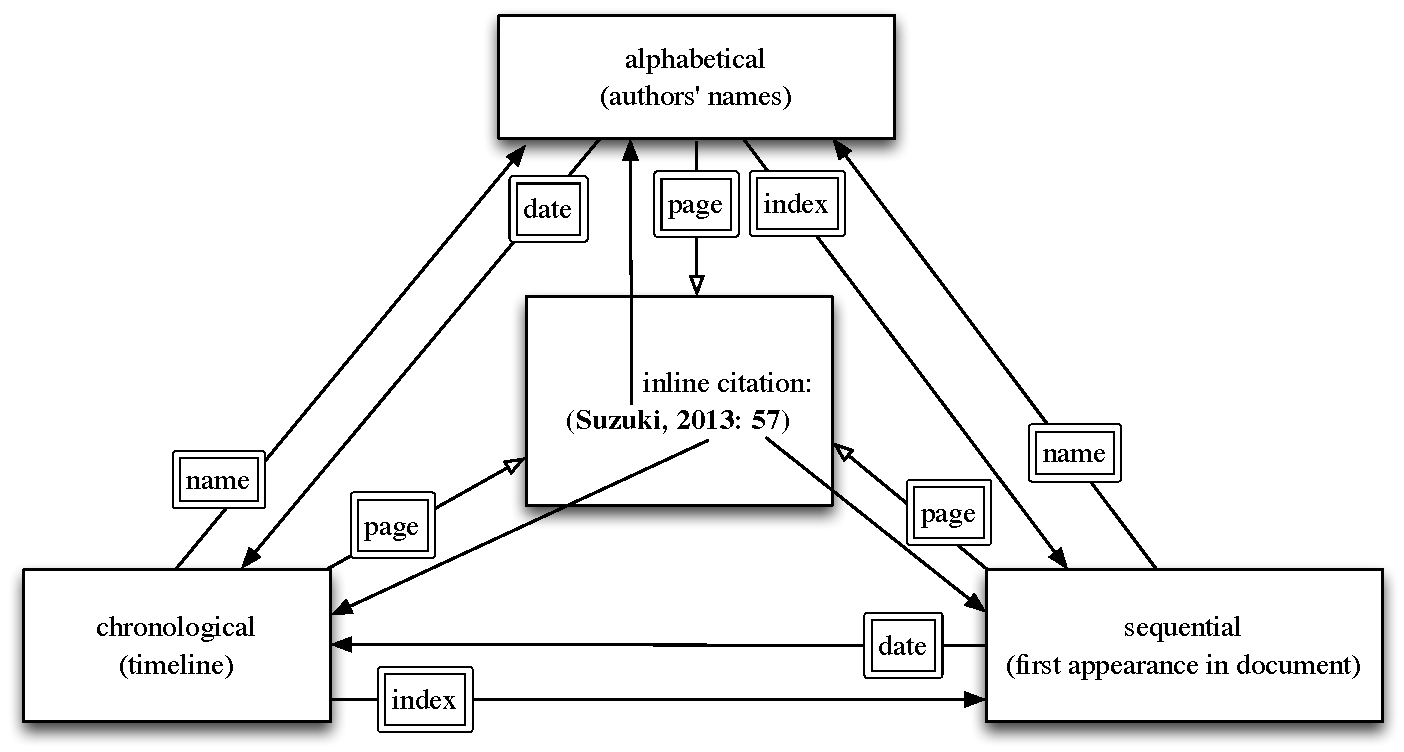
\includegraphics[width=\textwidth]{figure.pdf}
\caption{Hyperreferential links across document and among the multibibliographies:
Each inline citation, 
exemplified by the block in the center,
is linked to references in three subbibliographies,
which are cross-linked to each other
and can also be linked back to the inline callout.
Hollow arrowheads represent links provided by \texttt{backref};
solid arrowheads represent links provided by the \texttt{multibibliography} package.}
\label{fig-multibibliography}
\end{center}
\end{figure*}

This multibibliography system is copotentiated by the hypertextual \texttt{hyperref}\footnote{\url{www.ctan.org/pkg/hyperref}} package.
When using them together with an appropriate viewer or browser (such as \texttt{xdvi}, \texttt{acrobat}, or Adobe Reader),
clicking an inline citation
jumps to the respective entry in one of the reference lists.
%Further refinements suggested themselves,
As illustrated by Fig.\,\ref{fig-multibibliography},
the \texttt{multibibliography} inline \texttt{hyperref} hotspot is articulated to allow clicking on
\begin{description}
\item[the name,] which jumps to the corresponding entry in the alphabetical bibliography;
\item[the index number,] which jumps to the respective entry in the sequential bibliography; or
\item[the date,] which jumps to the matching entry in the chronological bibliography.
\end{description}

Similarly,
cross-references among the respective sub-bibliographies are also hyperlinked,
although from the labels, and not the \texttt{bibitem} bodies of the citations.
%(since it seemed too difficult to program).
The ``\texttt{[backref=page]}'' \texttt{hyperref} extension\footnote{\url{www.tug.org/applications/hyperref/manual.html}} is also compatible,
generating the familiar and useful back-references in all three subbibliographies:
lists of clickable page number links 
associated with each entry in the bibliography
pointing back to the respective citations
(excepting those generated by \texttt{nocites}).
The generation of these back-references,
indicated by the hollow arrowheads in Fig.\,\ref{fig-multibibliography},
represents ``closing the loop'' on the fully crossed relation set.

We have not yet experimented with combining this package with other bibliographic packages
\cite{Patashnik:bibtexing}
such as \texttt{natbib}\footnote{\url{www.ctan.org/pkg/natbib}}
or \texttt{chapterbib}\footnote{\url{www.ctan.org/pkg/chapterbib}} \cite[p.\,217--221]{kopka03}.

\section{Implications}

The extended inline citation style was designed for the multibibliography,
but can be deployed and is useful even without it.
The bibliographic dilation is perhaps more appropriate or at least more appealing for electronic dissemination,
as traditional print-based publishers might resent the cost of extra pages.
The fully crossed hyperreferential links are a convenient way of establishing the context of references,
seamlessly expressing citations' appearances in the document and in time.

Maybe the three ``slices'' through the bibliographic database that we have organized suffice for most ordinary publishing,
but presumably someone could make even more styles of bibliographic lists,
corresponding to special purposes,
sorted by attributes such as
number of authors,
number of pages,
conference or journal,
location,
etc.
The philosophy is to leverage the power of hyperreferential idioms to augment reading
by considering a document as a special kind of database
that is indexed in appropriate dimensions,
especially including the name--value pairs in its associated bibliographic information
(such as that captured by \texttt{bibtex} files)
plus derived information available after compilation
(such as sequence number and appearance location).

In the future,
the date should be articulated to add the month to the \texttt{sort.label} in the presort \texttt{FUNCTION}
in the \texttt{chronological.bst} file,
since it isn't one of the built-in keys of the \texttt{makebst} package
\cite{Markey:Tame_the_BeaST},
as the merlin system didn't anticipate such fine-grained sortings.
As \cite[p.\,13]{Markey:Tame_the_BeaST} observes,
the month is somewhat problematic,
since it is indicated by a character string,
but is really an ordinal.
If built-in macros (``\texttt{jan}'', ``\texttt{feb}'', etc.) are used,
they can be easily mapped to months and used for sorting,
but if, as is often the case, the field is reinterpreted to mean date
(bimonthly publications indicated by something like \texttt{month = "March \& April"},
quarterly dates as \texttt{month = "Autumn"}, etc.),
this scheme will not easily generalize.

It is our hope that old-fashioned conventions,
established in the context of technological restrictions that have now been overcome,
may be relaxed.
We find this multidimensional presentation useful,
are adopting it at the first author's university as a recommended style for masters theses and doctoral dissertations,
and hereby encourage other institutions to emulate this innovation,
especially for extended works
such as monographs and books.

%\bibliographystyle{apalike}
%\begin{thebibliography}{99} 
%
%\bibitem[Kopka and Daly, 2003: 2]{kopka03}
% Kopka, H. and Daly, P.~W. (2003). 
%\newblock {\em Guide to LaTeX}. 
%\newblock Number~0. Addison-Wesley Professional, 4th edition. 
%
%\bibitem[Mori, 2009: 3]{Mori:Managing_bibliographies}
% Mori, L.~F. (2009). 
%\newblock Managing bibliographies with {\LaTeX}. 
%\newblock {\em TUG: {\TeX} Users Group Meeting}, 30:36--48. 
%
%\bibitem[Patashnik, 1998: 1]{Patashnik:bibtexing}
% Patashnik, O. (1998). 
%\newblock Bib{\TeX}ing. 
%\newblock \url{http://mirrror.ctan.org/biblio/bibtex/contrib/doc/btxdoc.pdf}. 
%
%\end{thebibliography} 

%\bibliographystyle{apalike}
%\bibliography{type}

\renewcommand\refname{References sorted by name}
\bibliographystyle{apalike}
%%\addcontentsline{toc}{chapter}{References sorted by name}
\bibliography{type}
%
%%\clearpage
\renewcommand\refname{References sorted by appearance}
%%\addcontentsline{toc}{chapter}{References sorted by appearance}
\bibliographysequence{type}
%%
%%\clearpage
\renewcommand\refname{References sorted by year}
%%\addcontentsline{toc}{chapter}{References sorted by year}
\bibliographytimeline{type}

\makesignature
\end{document}